\documentclass{csbulletin}
\usepackage[utf8]{inputenc}
\usepackage[usenames,dvipsnames,svgnames,table]{xcolor}
\usepackage{tabularx}
\usepackage{booktabs}
\usepackage{pgfplots}
\usepackage{amsmath}
\usepackage[all]{nowidow}
\pgfplotsset{compat=1.8}
\usepgfplotslibrary{statistics}
\usepackage{hologo}
\usepackage{url}
% Apply the `\@cline` and `\@@@cmidrule` patch.
\usepackage{regexpatch}
\makeatletter
\xpatchparametertext\@@@cmidrule{-}{\cA-}{}{}
\xpatchparametertext\@cline{-}{\cA-}{}{}
\makeatother
\begin{document}
  \selectlanguage{english}
  \title{The trends in the usage of \TeX\ for the preparation of
    theses and dissertations at the Masaryk University in Brno}
  \EnglishTitle{The trends in the usage of \TeX\ for the
    preparation of theses and dissertations at the Masaryk
    University in Brno}
  \author{Vít Novotný}
  \podpis{Vít Novotný\\witiko@mail.muni.cz}
  \maketitle

  {\def\theAbstract{%
    This article is a statistical analysis of theses and
    dissertations written and defended during 2010--2015 at the
    Masaryk University in Brno (MU). The author assesses the trends
    in the usage of \TeX\ and tests the hypothesis that theses and
    dissertations written using \TeX\ were rated significantly
    better than those not written using \TeX.
    \medskip\par\keywords:\smallskip\par\noindent
    thesis, dissertation, statistics}

  \begin{abstract}\theAbstract\end{abstract}

  % A redefinition of the tabular environment
  \let\oldtabularx\tabularx
  \let\oldendtabularx\endtabularx
  \def\tabularx{\rowcolors{1}{}{black!8}\oldtabularx}
  \def\endtabularx{\oldendtabularx}
  \def\cellemph{\cellcolor{white!70!yellow}}
  % Adjust measurements
  \setlength{\aboverulesep}{0pt}
  \setlength{\belowrulesep}{0pt}
  \setlength{\extrarowheight}{.75ex}

  \section{Introduction}
  A statistical analysis of theses defended at the Masaryk
  University in Brno (MU) between 2010 and 2015 was carried out by
  the author of this article. The sample data for the analysis were
  kindly provided by doc. Ing. Michal Brandejs, CSc., the head of
  the Computer Systems Unit at the Faculty of Informatics at MU.

  \begin{table}
    \begin{tabularx}{\textwidth}{Xrr}
      \textbf{Faculty} & \textbf{\#} & \textbf{\%} \\
      \toprule
      Arts                         & $10\,000$ & $21.98$ \\% 1421
      Education                    & $8\,219$  & $18.07$ \\% 1441
      Social Studies               & $5\,599$  & $12.31$ \\% 1423
      Science                      & $5\,275$  & $11.60$ \\% 1431
      Law                          & $4\,824$  & $10.60$ \\% 1422
      Economics \& Administration  & $4\,591$  & $10.09$ \\% 1456
      Informatics                  & $2\,904$  &  $6.38$ \\% 1433
      Sports Studies               & $2\,062$  &  $4.53$ \\% 1451
      Medicine                     & $2\,014$  &  $4.43$ \\% 1411
      \bottomrule
      \textbf{Total}     & $\mathbf{45\,488}$ & $\mathbf{100.00}$
    \end{tabularx}
    \caption{The distribution of theses defended during 2010--2015
      across the faculties of MU}
    \label{table:statistics-faculty}
  \end{table}

  Table \ref{table:statistics-faculty} details the distribution of
  theses written and defended during 2010--2015 across the
  faculties of MU and Table \ref{table:statistics-tex} illustrates
  how many of these theses were written using \TeX. Table
  \ref{table:statistics-tex-yearly} then details the trends in the
  usage of \TeX\ by the students of bachelor's, master's and
  doctoral degree programmes at the Faculty of Informatics (FI) and
  the Faculty of Science (Sci).  Other faculties of MU were not
  considered, since the number of theses written at them using
  \TeX\ was statistically insignificant (see Table
  \ref{table:statistics-tex}). Theses written by students of
  lifelong education programmes were likewise ignored, since none
  of them were written using \TeX.

  \begin{table}
    \begin{tabularx}{\textwidth}{Xrrr}
      \textbf{Faculty} & \textbf{With \TeX} & \textbf{Total} &
      \textbf{\%} \\
      \toprule
      Informatics                 & $1\,716$ & $2\,904$  &
      $59.09$ \\% 1433
      Science                     & $786$     & $5\,275$  &
      $14.90$ \\% 1431
      Economics \& Administration & $64$      & $4\,591$  &
      $1.39$  \\% 1456
      Arts                        & $69$      & $10\,000$ &
      $0.69$  \\% 1421
      Medicine                    & $8$       & $2\,014$  &
      $0.40$  \\% 1411
      Law                         & $15$      & $4\,824$  &
      $0.31$  \\% 1422
      Education                   & $19$      & $8\,219$  &
      $0.23$  \\% 1441
      Social Studies              & $12$      & $5\,599$  &
      $0.21$  \\% 1423
      Sports Studies              & $3$       & $2\,062$  &
      $0.15$  \\% 1451
      \bottomrule
      \textbf{Total} & $\mathbf{2\,692}$ & $\mathbf{45\,488}$ &
      $\mathbf{5.92}$
    \end{tabularx}
    \caption{The distribution of theses written using \TeX,
      which were defended during 2010--2015 across the faculties of
      MU}
    \label{table:statistics-tex}
  \end{table}

  \begin{table}
    \begin{tabularx}{\textwidth}{Xlrrrrrr}
      \textbf{Degree} & \textbf{Fac.} & \textbf{2010} &
      \textbf{2011} & \textbf{2012} & \textbf{2013} & \textbf{2014}
      & $R$\\
      \toprule
      Bachelor's
        & FI  & $58.92$ & $59.44$ & $49.54$ & $53.77$ &
          $59.06$ & \textcolor{red}{$-0.195$} \\
        & Sci & $11.55$ & $13.00$ & $15.90$ & $19.79$ &
          $15.16$ & \textcolor{OliveGreen}{$+0.703$} \\
        & All & $5.08$ & $6.19$ &
          $6.00$ & $6.08$ & $6.24$ &
          \textcolor{OliveGreen}{$+0.731$} \\ \midrule
      Master's
        & FI  & $60.61$ & $59.91$ & $60.08$ & $64.50$ &
          $57.96$ & \textcolor{red}{$-0.046$} \\
        & Sci & $19.38$ & $13.54$ & $13.75$ & $13.78$ &
          $17.71$ & \textcolor{red}{$-0.180$} \\
        & All & $6.02$ & $4.88$ &
          $5.22$ & $6.59$ & $6.29$ &
          \textcolor{OliveGreen}{$+0.490$} \\ \midrule
      Doctoral
        & FI  & $100.00$ & $76.67$ & $71.88$ & $83.87$ &
          $90.91$ & \textcolor{red}{$-0.155$} \\
          \cline{2-8}\cellcolor{white}
        & \multicolumn{1}{|l}{\cellemph Sci} & \cellemph$18.09$ &
          \cellemph$10.71$ & \cellemph$12.75$ & \cellemph$10.19$ &
          \cellemph$8.85$ & \multicolumn{1}{r|}{\cellemph
          \textcolor{red}{$-0.830$}} \\ \cline{2-8}
        & All & $8.83$ & $8.23$ &
          $8.41$ & $9.38$ & $7.43$ &
          \textcolor{red}{$-0.361$} \\
        \bottomrule
      \textbf{All}
        & \textbf{FI } & $\mathbf{60.83}$ &
          $\mathbf{60.53}$ & $\mathbf{54.92}$ & $\mathbf{60.57}$ &
          $\mathbf{59.34}$ & \textcolor{red}{$\mathbf{-0.188}$} \\
        & \textbf{Sci} & $\mathbf{14.86}$ &
          $\mathbf{12.96}$ & $\mathbf{14.74}$ & $\mathbf{16.55}$ &
          $\mathbf{15.45}$ &
          \textcolor{OliveGreen}{$\mathbf{+0.577}$} \\
          \cline{2-8}\cellcolor{white}
        & \multicolumn{1}{|l}{\cellemph\textbf{All}} & \cellemph$\mathbf{5.67}$ &
          \cellemph$\mathbf{5.70}$ & \cellemph$\mathbf{5.73}$ &
          \cellemph$\mathbf{6.41}$ & \cellemph$\mathbf{6.28}$ &
          \multicolumn{1}{r|}{\cellemph\textcolor{OliveGreen}{$\mathbf{+0.855}$}}
          \\ \cline{2-8}
    \end{tabularx}
    \caption{The percentage of theses written using \TeX\ 
      which were defended in each year during 2010--2014 and the
      sample correlation coefficient $R$ between the percentage and
      the years with remarkably strong correlations emphasized}
    \label{table:statistics-tex-yearly}
  \end{table}

  \section{Analysis}
  A thesis was considered to be written using \TeX, if one
  or more files submitted with it satisfied one or more of the
  following conditions: \begin{itemize}
    \item The suffix was \texttt{tex}.
    \item The magic number was that of a DVI file.
    \item The MIME type was \texttt{application/postscript} and
      the file contained the \texttt{TeXDict} substring suggesting
      that the file was a PostScript document, which had been created
      using the \textsf{dvips} utility.
    \item The MIME type was \texttt{application/pdf} and either
      the \texttt{Creator} or the \texttt{Producer} PDF
      header contained the \texttt{TeX} substring suggesting that
      the file had been created using either the \textsf{dvipdfm}
      utility or a \TeX\ engine, which supports PDF output.
  \end{itemize} Provided the heuristic is sound, there was a marked
  and steady increase in the use of \TeX\ for the typesetting
  of theses at MU during 2010--2014 (see Table
  \ref{table:statistics-tex-yearly}). This, however, does not
  necessarily hold true for individual faculties and degree study
  programmes with some of them showing barely any correlation
  between the years and the use of \TeX\ and others showing a
  strong negative correlation. A particularly striking example of
  the latter is the pronounced downwards trend in the use of
  \TeX\ for the typesetting of doctoral theses at Sci.

  \begin{table}
    \begin{tabularx}{\textwidth}{Xrrrrr}
      &\textbf{Without \TeX}&E(\textbf{With \TeX})
      &O(\textbf{With \TeX})&$(\rm{E}-\rm{O})^2/\rm{E}$
      \\ \toprule
      \textbf{\parbox[t]{1em}{\centering A}} 
        &$15\,476$&$987.635$&\textcolor{OliveGreen}{$1\,181$}&
        $37.858$\\
      \textbf{\parbox[t]{1em}{\centering B}}
        &$9999$&$638.108$&\textcolor{red}{$587$}&$4.093$\\
      \textbf{\parbox[t]{1em}{\centering C}}
        &$7\,926$&$505.815$&\textcolor{red}{$381$}&$30.799$\\
      \textbf{\parbox[t]{1em}{\centering D}}
        &$4\,020$&$256.545$&\textcolor{red}{$194$}&$15.248$\\
      \textbf{\parbox[t]{1em}{\centering E}}
        &$2\,783$&$177.603$&\textcolor{red}{$128$}&$13.853$\\
      \textbf{\parbox[t]{1em}{\centering F}}
        &$1\,979$&$126.294$&\textcolor{OliveGreen}{$145$}&
        $2.771$\\
      \bottomrule
      \textbf{Total} &$\mathbf{42\,183}$&$\mathbf{2\,692}$&
        $\mathbf{2\,692}$&$\mathbf{104.623}$
    \end{tabularx}
    \caption{The contingency table of the numbers of marks awarded
      to theses written and defended during 2010--2015 with
      Pearson's goodness-of-fit measure
      $(\rm{E}-\rm{O})^2/\rm{E}$ between the expected (E)
      and the observed (O) numbers of marks awarded to theses
      written using \TeX}
    \label{table:statistics-contingency}
  \end{table}

  \begin{figure}
    \centering
    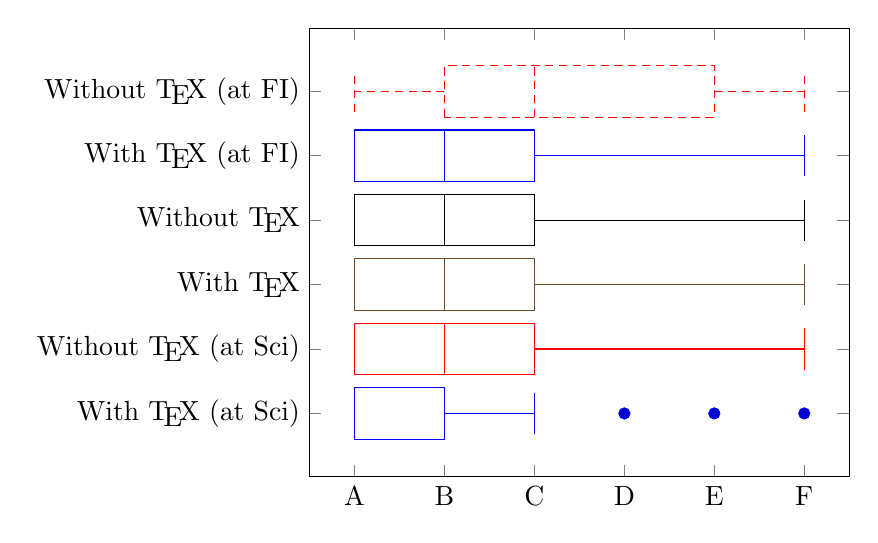
\begin{tikzpicture}
      \begin{axis}
        [
          ytick={1,2,3,4,5,6},
          xticklabels={,,A,B,C,D,E,F},
          yticklabels={With \TeX{} (at Sci),
                       Without \TeX{} (at Sci),
                       With \TeX{},
                       Without \TeX{},
                       With \TeX{} (at FI),
                       Without \TeX{} (at FI)},
        ]
        \addplot+[
          boxplot prepared={
            lower quartile=1,
            median=1,
            upper quartile=2,
            upper whisker=3,
            lower whisker=1,
          },
        ] table[row sep=\\,y index=0] {
          data\\ 4\\ 5\\ 6\\
        };
        \addplot+[
          boxplot prepared={
            lower quartile=1,
            median=2,
            upper quartile=3,
            upper whisker=6,
            lower whisker=1,
          },
        ] table[row sep=\\,y index=0] {
          data\\
        };
        \addplot+[
          boxplot prepared={
            lower whisker=1,
            lower quartile=1,
            median=2,
            upper quartile=3,
            upper whisker=6,
          },
        ] table[row sep=\\,y index=0] {
          data\\
        };
        \addplot+[
          boxplot prepared={
            lower whisker=1,
            lower quartile=1,
            median=2,
            upper quartile=3,
            upper whisker=6,
          },
        ] table[row sep=\\,y index=0] {
          data\\
        };
        \addplot+[
          boxplot prepared={
            lower whisker=1,
            lower quartile=1,
            median=2,
            upper quartile=3,
            upper whisker=6,
          },
        ] table[row sep=\\,y index=0] {
          data\\
        };
        \addplot+[
          boxplot prepared={
            lower whisker=1,
            lower quartile=2,
            median=3,
            upper quartile=5,
            upper whisker=6,
          },
        ] table[row sep=\\,y index=0] {
          data\\
        };
      \end{axis}
    \end{tikzpicture}
    \caption{A box plot of the grades of theses written and
      defended during 2010--2015 at FI, Sci
      and all the faculties of MU with and without
      \TeX}
    \label{fig:statistics-grades}
  \end{figure}

  Suppose the null hypothesis $h_1$ that the grades awarded
  to theses written using and not using \TeX, respectively,
  have the same distribution on the significance level
  $\alpha=0.05$. The one-tailed Pearson's $\chi^2$ test
  \cite{Pearson00} of the goodness of fit was applied to the
  observations of awarded grades (see Table
  \ref{table:statistics-contingency}). Since \begin{equation}
    \sum_{\rm{A},\rm{B},\ldots,\rm{F}}
    (\rm{E}-\rm{O})^2/\rm{E}=104.623\gg11.07=
    \chi_{1-\alpha}^2(5)
  \end{equation} the author refused the null hypothesis $h_1$
  and concluded that the grades are indeed differently
  distributed on the significance level $\alpha$.

  Having shown that the distribution of grades awarded to theses
  written using and not using \TeX\ is different, the author
  proceeded to inspect, if this holds for individual grades.
  Suppose the null hypothesis $h_{\rm{A}}$ that the
  distribution of grade A being awarded to theses written using
  and not using \TeX is equivalent. The two-tailed
  Mann-Whitney U test~\cite{mann47} was applied to the
  observations of grade A being and not being awarded to theses
  written using and not using \TeX: \begin{align}
    \tag{Without \TeX\ (grade A)} m_1 &= 15\,476 \\
    \tag{With \TeX\ (grade A)}    m_2 &= 1\,181  \\
    \tag{Without \TeX\ (total)} n_1 &= 42\,183 \\
    \tag{With \TeX\ (total)}    n_2 &= 2\,692  \\
    U_1 &=  m_1(m_2\cdot0.5+(n_2-m_2))+
                  (n_1-m_1)((n_2-m_2)\cdot0.5) \\
      \nonumber&=52\,699\,952.5 \\
    U_2 &=  m_2(m_1\cdot0.5+(n_1-m_1))+
                  (n_2-m_2)((n_1-m_1)\cdot0.5) \\
      \nonumber&=60\,856\,683.5 \\
    U &= \min(U_1,U_2) = U_1 = 52\,699\,952.5
  \end{align} Since $n_1n_2\gg20$,
  $U\sim\text{N}\left(\frac{n_1n_2}2,
  \frac{n_1n_2(n_1+n_2+1)}{12}\right)$. After normalization to
  \begin{equation}
    \text{N}(0,1)\sim z =
    \frac{U-\frac{n_1n_2}2}{\sqrt{\frac{n_1n_2(n_1+n_2+1)}{12}}}
    \approx-\frac{4\,078\,365.5}{651\,662.46}\approx-6.258
  \end{equation} the two-tailed $p$-value $\beta$ was computed by
  the author as follows:\begin{align}
    & \operatorname{arg\,min}\limits_{\beta} P(\Phi^{-1}_{\beta/2}
        \leq z\leq\Phi^{-1}_{1-\beta/2})=\beta \\
    \nonumber& \iff\Phi^{-1}_{\beta/2}=-6.258 \iff\beta/2=1-
        \Phi(6.258)\iff\beta\approx 0
  \end{align}Since $\beta<\alpha$, the author refused the null
  hypothesis $h_\text{A}$ on the significance level $\alpha$.
  Following a similar procedure for marks B--F, the author arrived
  at the following conclusions on the significance level $\alpha$:
  \begin{itemize}
    \item Theses written using \TeX\ had been awarded grade A
      significantly more often than theses not written using \TeX.
    \item Theses written using \TeX\ had been awarded grades C and
      D significantly less often than theses not written using
      \TeX.
    \item No significant difference was observed in the
      distributions of grades B, E and F being awarded to theses
      written using and not using \TeX.
  \end{itemize}
  A box plot of the grades is shown in Figure
  \ref{fig:statistics-grades}.

  \section{Conclusion}
  The author has shown that there was a marked and steady increase
  in the usage of \TeX\ at MU during 2010--2014 and that the usage
  of \TeX\ correlated with statistically significantly better
  grades during 2010--2015.

  \begin{thebibliography}{9}
    \bibitem{Pearson00}
          Pearson,~Carl.
          \textit{``On the criterion that a given system of deviations from the probable in the case of a correlated system of
            variables is such that it can be reasonably supposed to have arisen from random sampling''}.
          In:~\textit{Philosophical Magazine} (1900), pp. 157--175.
    \bibitem{mann47}
          Mann,~H.~B. and Whitney, D.~R.
          \textit{``The generalization of `Student's problem' when several different population variances are involved''}.
          In:~\textit{The Annals of Mathematical Statistics} 18.1 (1947), pp. 50--60.
          \textsc{doi:}~\texttt{10.1214/aoms/1177730491}.
          \textsc{url:}~\url{http://dx.doi.org/10.1214/aoms/1177730491} (visited on 06/29/2015).
  \end{thebibliography}

  \begin{summary}\theAbstract\end{summary}}
\end{document}
